\chapter{Absence of Information is also Knowledge}

This chapter presents an approach to the problem of learning object placement habits of humans in an occluded environment. Generally in domestic environments like our home, we humans prefer to store our food, cooking equipment, silverware and dishes inside closed cabinets like drawers, cupboards and refrigerators. This causes high level of occlusion for data collection.

We assume there is a domestic service robot which while interacting in human environments records all the information generated using vision sensor.
So for a domestic robot with only camera as a sensor, the chances of observing  these objects inside closed cabinets is drastically reduced.

\begin{figure}[htp]
\centering
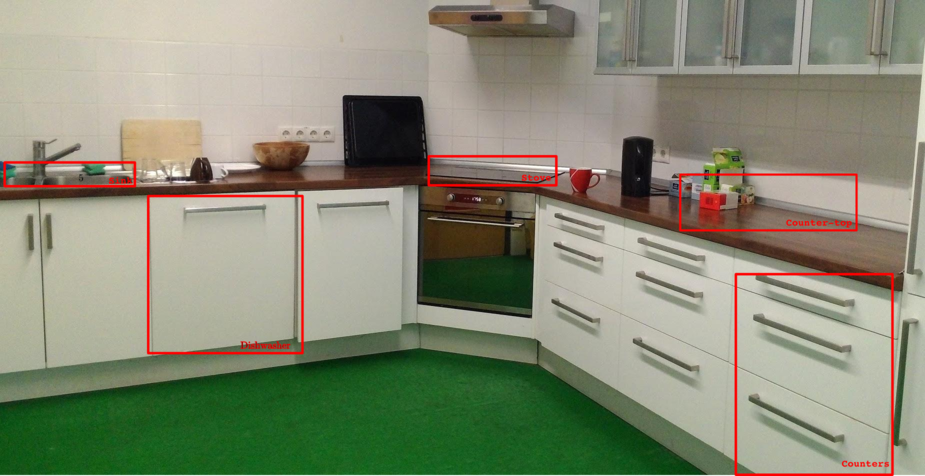
\includegraphics[width=0.8\textwidth]{images/kitchen_crop_ano.png}
\caption{Kitchen environment with occluded spaces}
\label{fig:kitchen occluded}
\end{figure}

The basic requirement of machine learning is data, from which information and knowledge can be learnt. But in highly occluded environments like kitchen its difficult for a domestic robot to make an observation of the object and record the object location.  Hence our hypothesis that we can learn knowledge about object locations quantitatively i.e. learning patterns from the data observed, becomes a herculean task to prove.

An alternative approach to counter the sparsity of data is by recording the absence of the object in visible locations and learning knowledge about where objects are not located. Consider an motivating example, as depicted in Figure \ref{fig:alllocations} . Here, a mobile robot is in a kitchen in the morning. The following locations can be scanned by the robot: kitchen-sink, counter-top and stove, while the cabinets, dishwasher and refrigerator are occluded. The robot will make observations of cup and kettle on counter-top , spoon on the sink top. Assume that the robot is also learning object locations of cooking pot. If the robot only records the observed objects then there is no data recorded for the cooking-pot and no knowledge is learned about the cooking-pot. \emph{A possible solution is to even record the \textbf{absence} of cooking-pot on the visible locations}. From this the robot can learn that the cooking-pot is less probable to be on the kitchen-sink, counter-top and stove during morning time. Supplementary the robot can also learn that there is higher probability for the cooking-pot being in the cabinet or dishwasher.

\begin{figure}
    \centering
    \begin{subfigure}[b]{0.3\textwidth}
        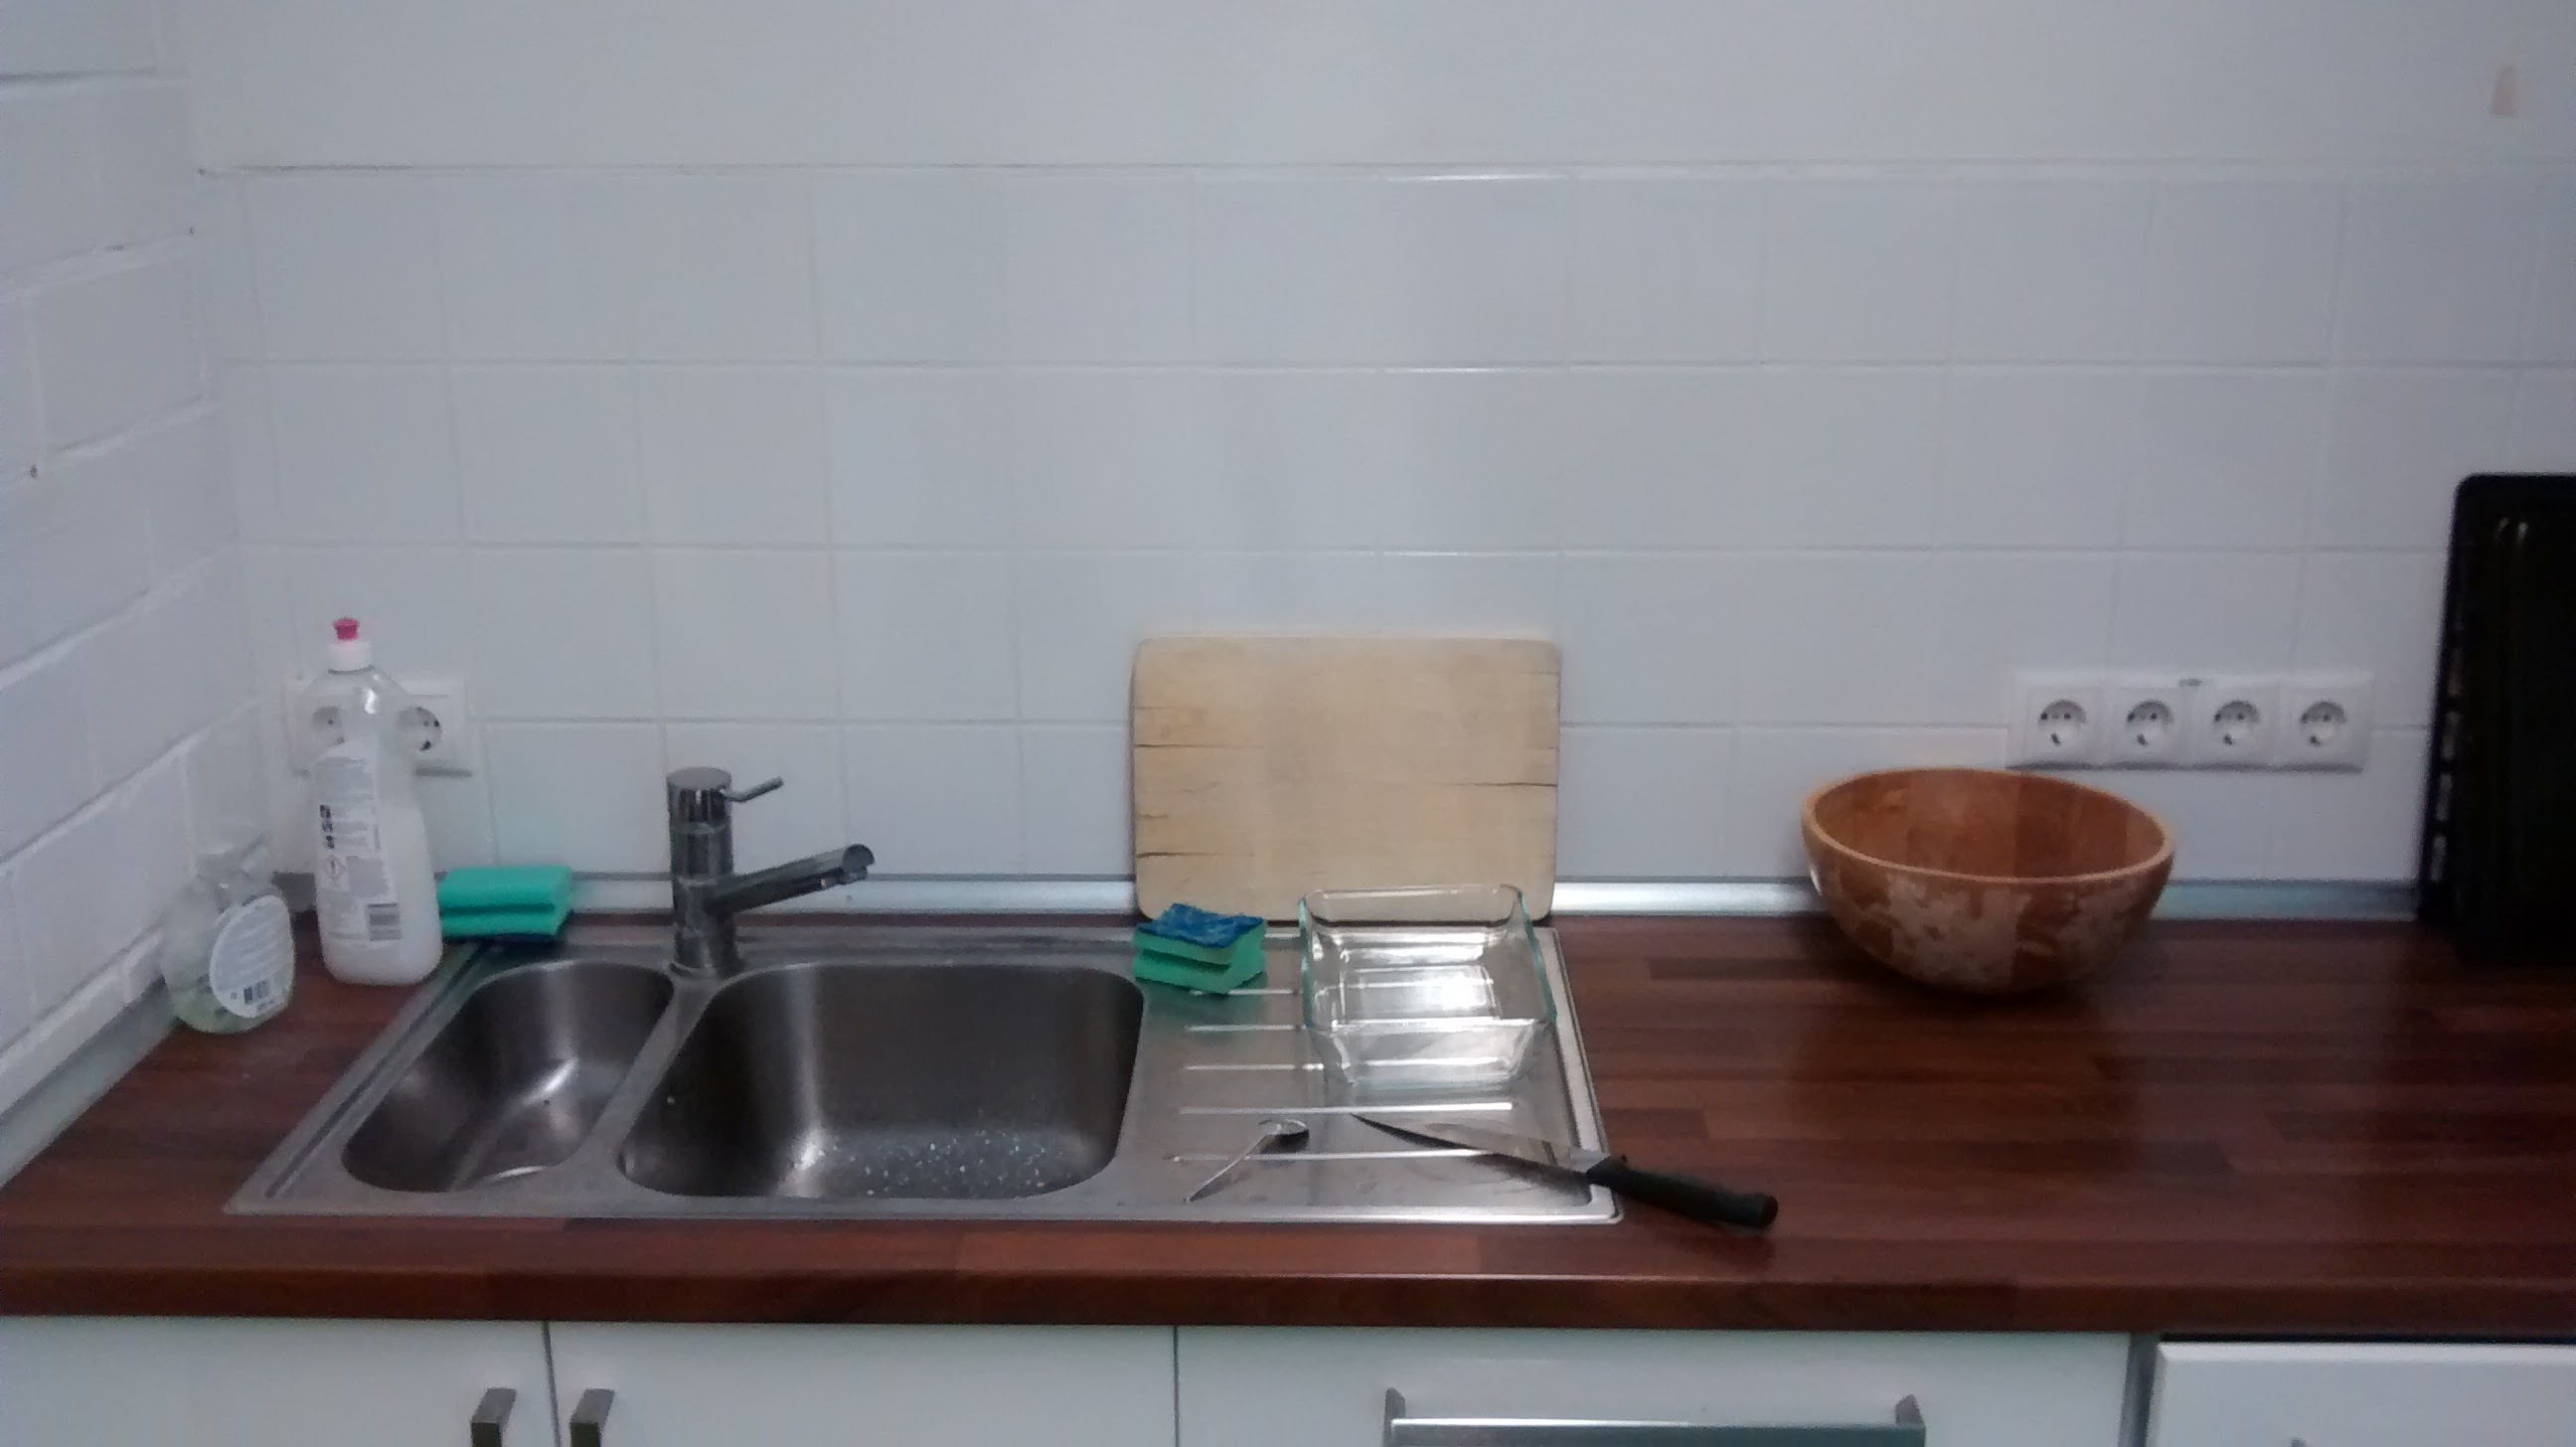
\includegraphics[width=\textwidth]{images/sink.jpg}
        \caption{Sink}
        \label{fig:sink}
    \end{subfigure}
    ~ %add desired spacing between images, e. g. ~, \quad, \qquad, \hfill etc. 
      %(or a blank line to force the subfigure onto a new line)
    \begin{subfigure}[b]{0.3\textwidth}
        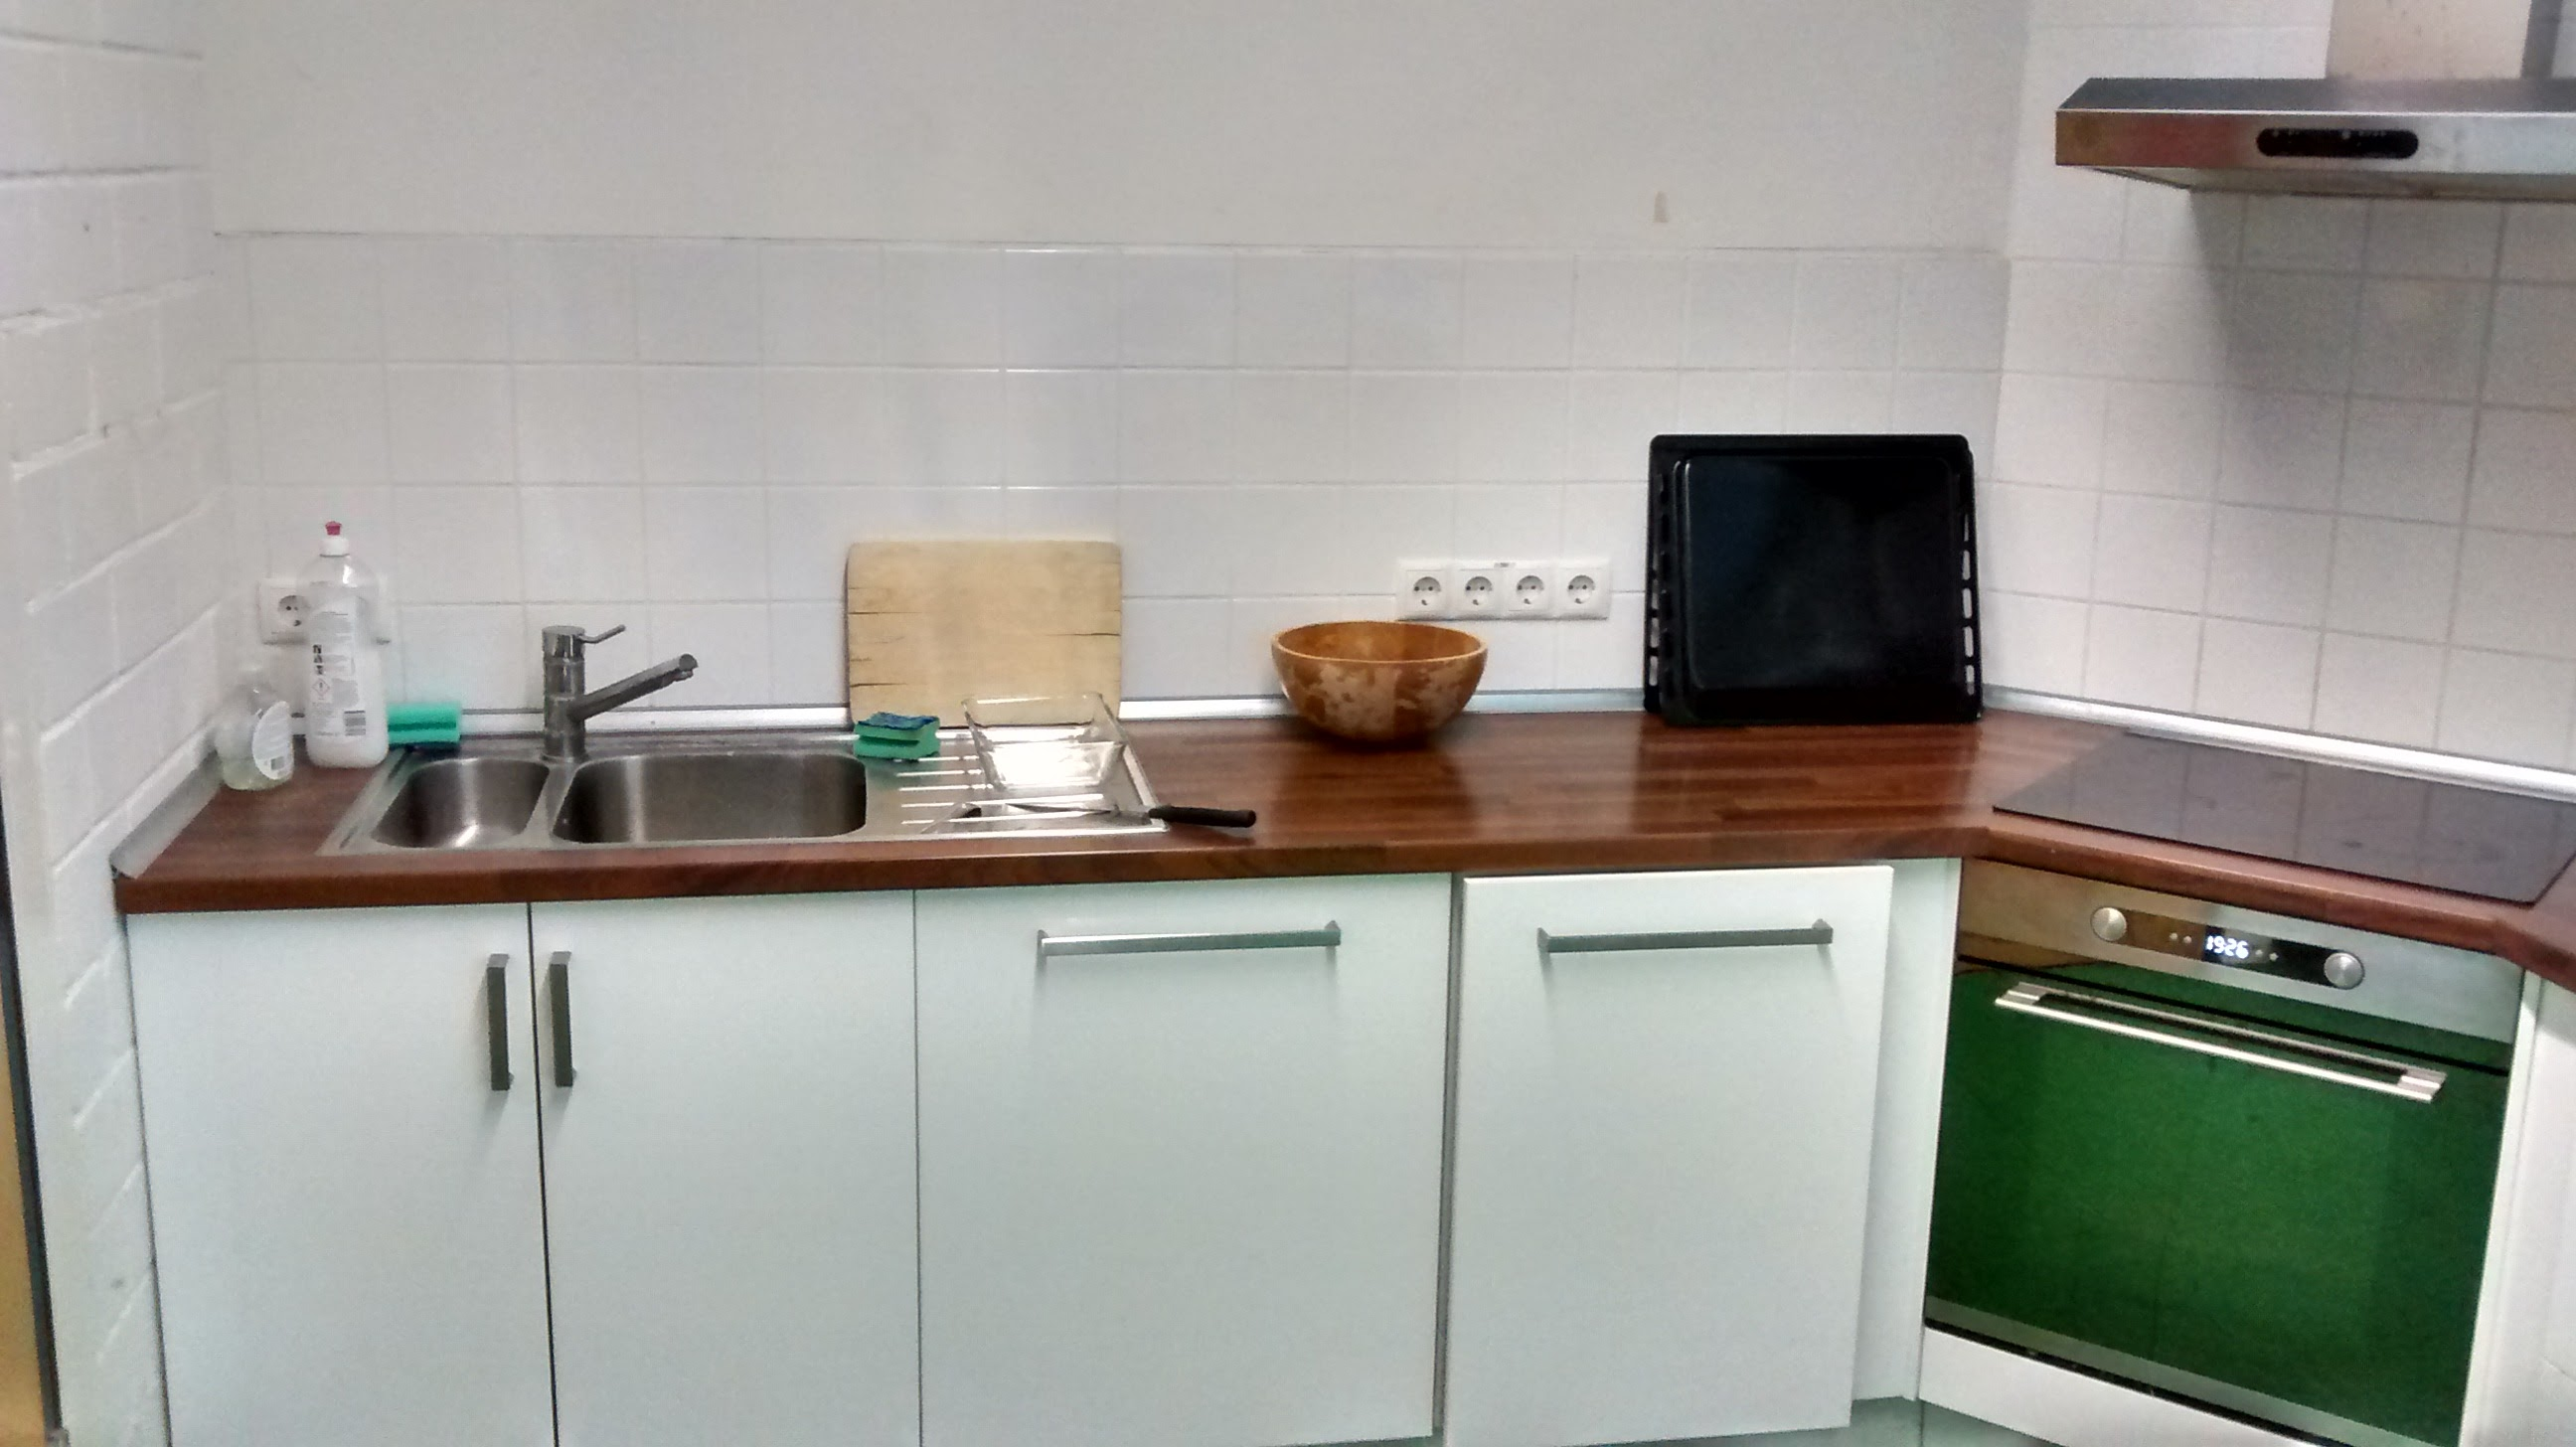
\includegraphics[width=\textwidth]{images/stove.jpg}
        \caption{Stove}
        \label{fig:stove}
    \end{subfigure}
    ~ %add desired spacing between images, e. g. ~, \quad, \qquad, \hfill etc. 
    %(or a blank line to force the subfigure onto a new line)
    \begin{subfigure}[b]{0.3\textwidth}
        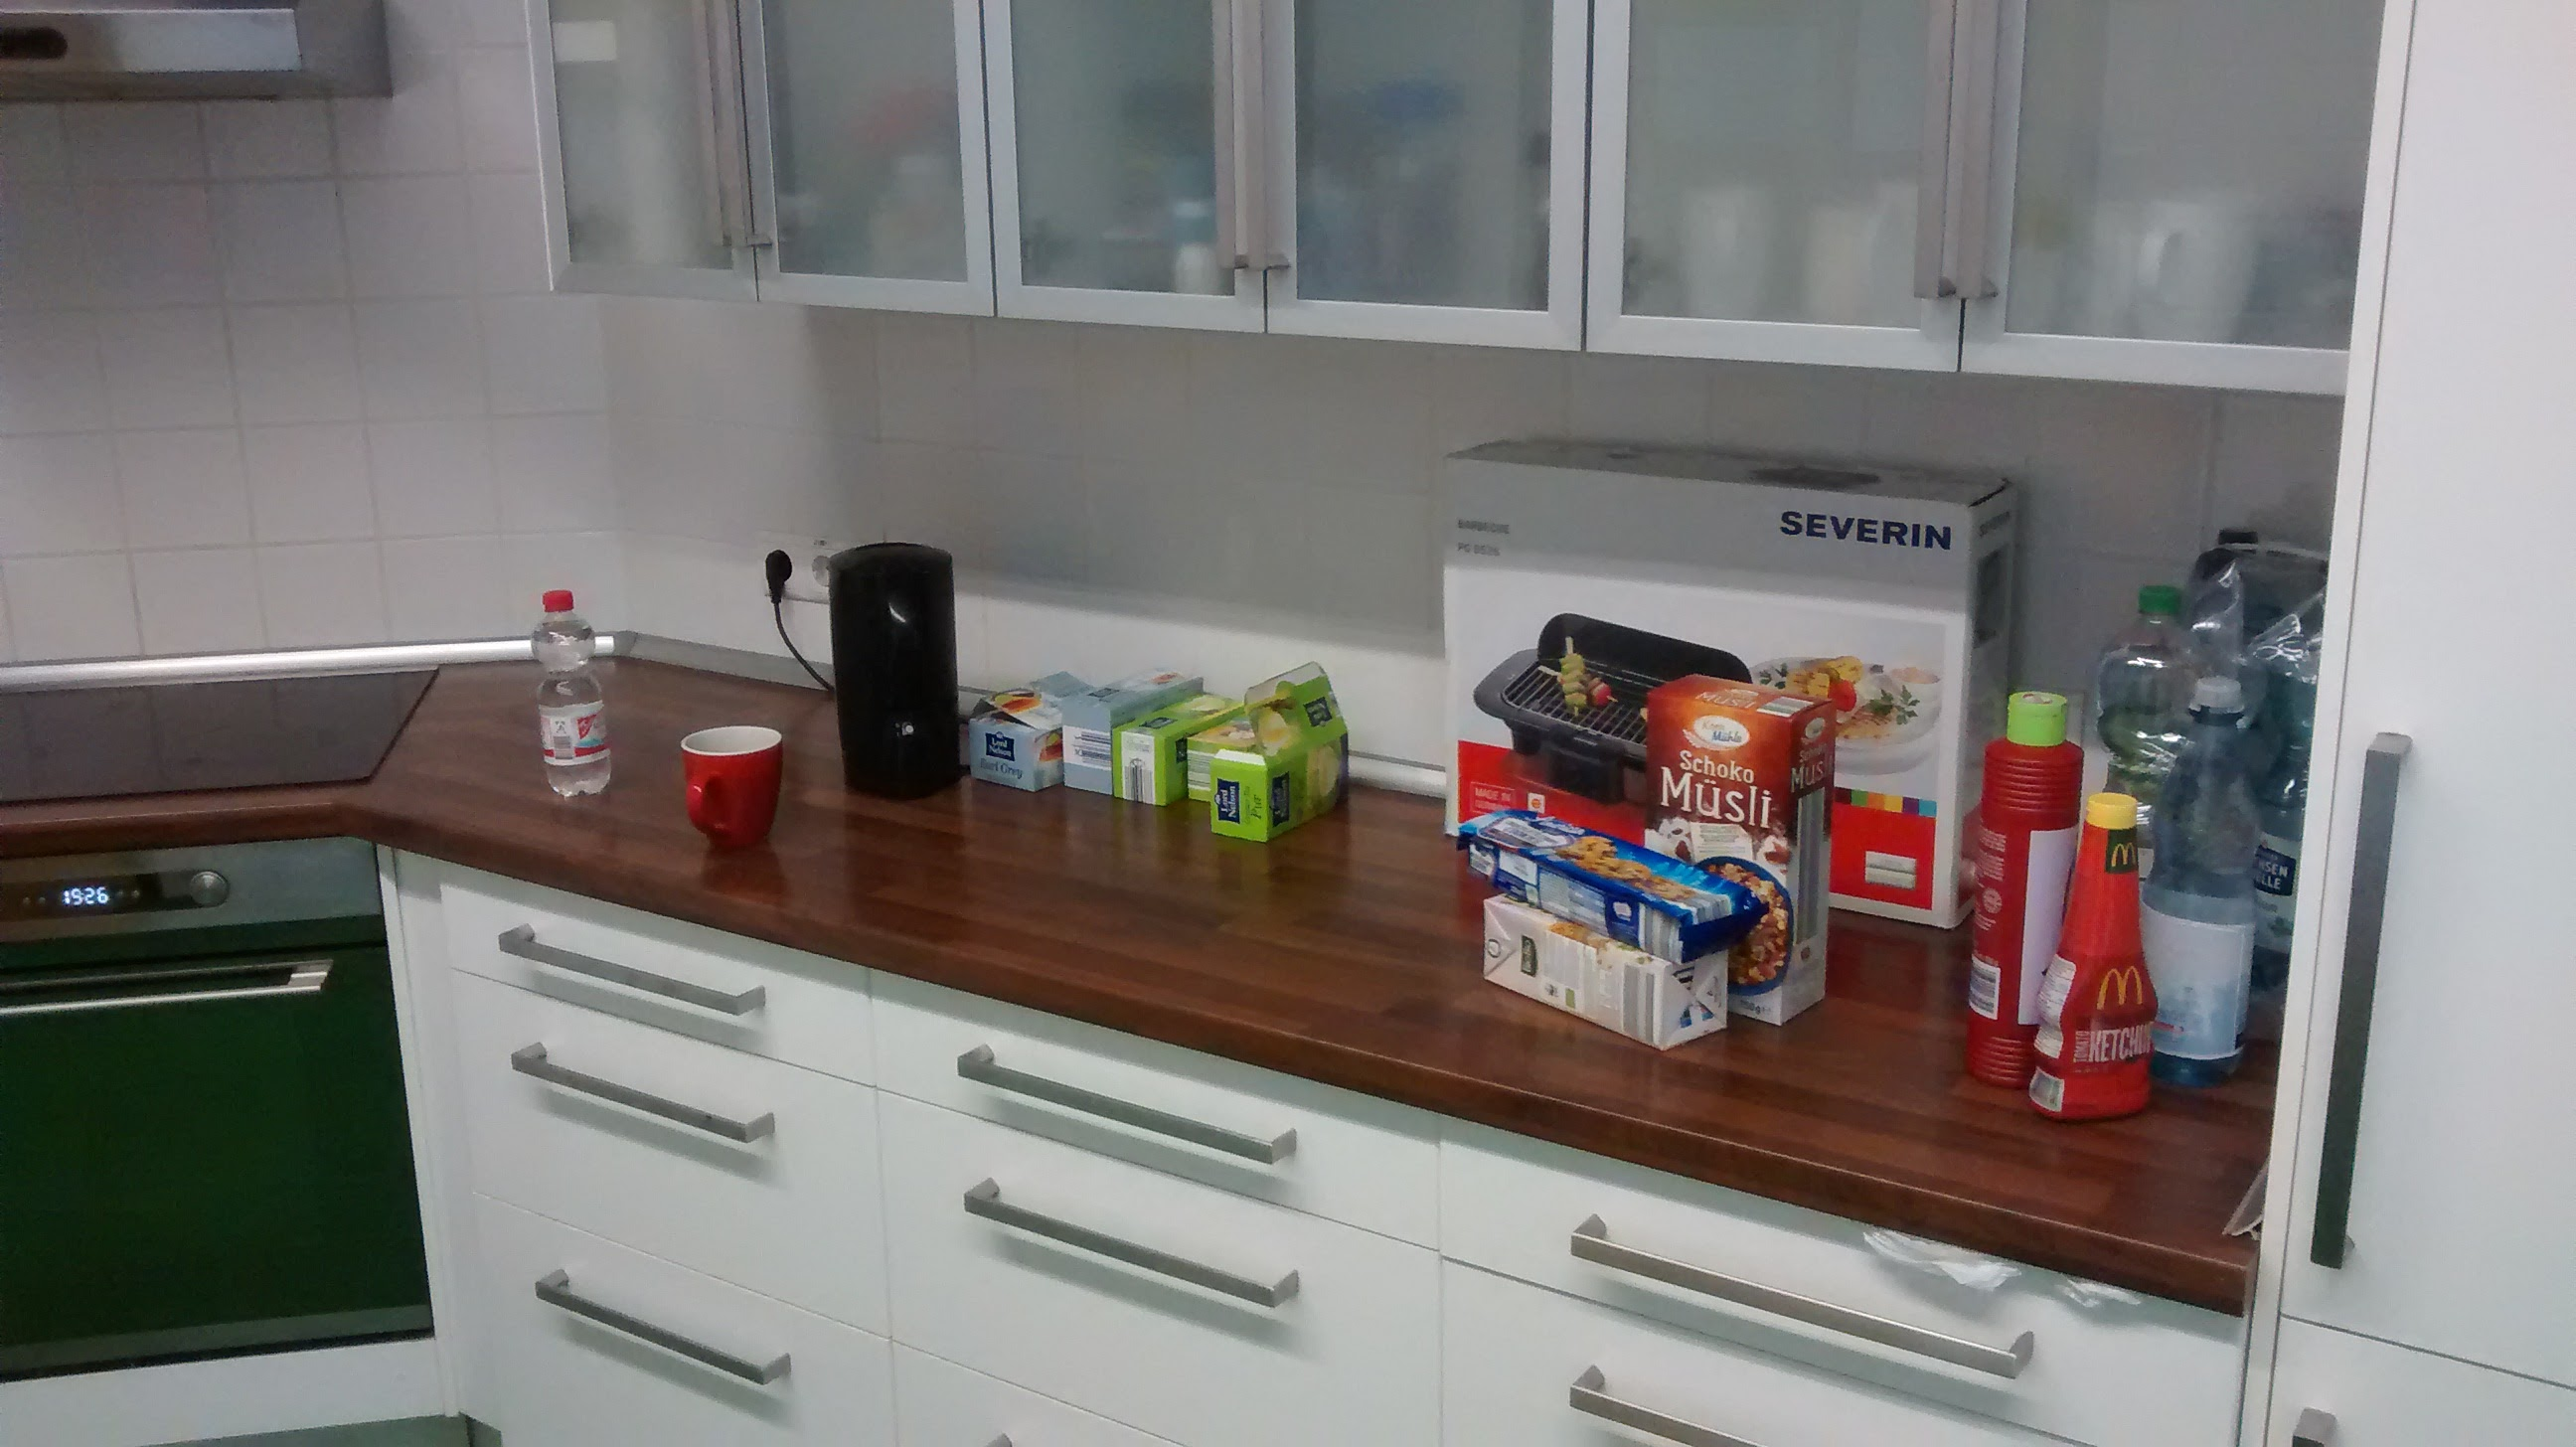
\includegraphics[width=\textwidth]{images/counter-top.jpg}
        \caption{counter-top}
        \label{fig:counter-top}
    \end{subfigure}
    \caption{Different possible object locations}\label{fig:alllocations}
\end{figure}


Thus models are developed which on absence of information of an object at a particular location decreases the probability of finding the object at that particular location while increasing the probabilities for other locations.


\FloatBarrier
\section{Dirichlet-Categorical-Bernoulli model}

For incorporating the absence observations we extended the Dirichlet-Categorical model  with a Bernoulli distribution.
In chapter \ref{} patterns in a single location were learned using a Beta-Bernoulli model, in chapter \ref{} we introduced the Dirichlet-Categorical model which could reason about multiple locations in single model, here we combine both the models. The Beta-Bernoulli model has the capability to learn from both success and failure results, this capability is added to the Dirichlet-Categorical model using a mixture node. 

The Bernoulli-trick is one way of making negative observations for certain location reduce its chances while making equally likely for the other locations. Thus, the location on which the object is not found are filtered out as impossible and the others are equally likely. The graphical diagram of the model is explained in \ref{dcbm}

The model is an extension as explained in \ref{sec: HDCM} . We combine a Bernoulli node $\gamma$ with the categorical node $x$. The Bernoulli is also an observation node as the categorical node. The observations are fed to the model to both the Bernoulli node and the categorical node. Suppose there are 3 locations where a object can be located. For a positive observation of locating the object at a location we feed [1.0 , 0.0, 0.0] to the Bernoulli node, where 1.0 represents object found at at location. For a negative observation i.e. the object not being found at a location the Bernoulli is given [0.0, 0.5, 0.5], where 0.0 signifies that no data was observed whereas the 0.5 increases uniformly the chances in the other locations.


\noindent
\begin{figure}[htp]
\qquad
\begin{minipage}{0.3\textwidth}
\centering

\tikz {
\node [const]                   (alpha) {$\alpha$};
\node [below=of alpha, latent]  (beta)  {$\beta$};
\node [below=of beta, latent]   (theta) {$\theta_i$};
\node [below=of theta, obs]     (x)     {$x_{ij}$};
\node [right=of x , xshift=0.05cm, obs]      (gamma) {$\gamma_{ij}$};
\edge {alpha} {beta};
\edge {beta} {theta};
\edge {theta} {x};
\edge {gamma} {x};
\plate {trials} {(x)(gamma)} {j location};
\plate {bags} {(theta)(x)(gamma)(trials)} {i time};
}

\end{minipage}%
\begin{minipage}{0.7\textwidth}

\begin{equation*}
	\alpha = <1, 1, .... , 1 > 
\end{equation*}
\begin{equation*}
	\beta \sim Dirichlet(\alpha)
\end{equation*}
\begin{equation*}
	\theta_i  \sim Dirichlet(\beta)
\end{equation*}
\begin{equation*}
	\gamma_{ij}  \sim Bernoulli(k)
\end{equation*}
\begin{equation*}
	x_{ij} \sim Categorical(\theta_i)
\end{equation*}
\end{minipage}

\caption[Dirichlet Categorical Bernoulli graphical model]{Graphical model representation of Dirichlet Categorical Bernoulli model. The boxes are ``plates" representing replicates. The outer plates represents hours of a day, while the inner plate represents if object was observed at the location each hour.}
\label{dcbm}
\end{figure}



\section{Experiments}

The goal of the experiments was to verify the performance of the proposed model with the HDCM introduce in \ref{}. 


The goal of the experiments was to comparatively evaluate the proposed method with the HDCM introduced in \ref{}, based on the number of experiments. For this we created a simulated dataset with known ground truth distributions. The observations were then by the models to learn the latent probabilities. The learned probabilities were then compared with the ground truth. The above experiments were run 
\subsection{Simulated Dataset: Kitchen Object Dataset}

To demonstrate the proposed approach we have generated a kitchen object dataset. The dataset consist of observations(presence and absence) of a cup in a kitchen environment made by a domestic robot. The robot can scan 4 locations in the kitchen: sink, counter-top, stove and cabinet. The time of the scan is discretized into 3 times of the day: morning, afternoon and night. 

The generative process for each possible observation(present and absent) in the dataset 
\begin{itemize}
    \item Choose $ \theta \sim Dirichlet(\alpha)$ (Distribution of object over location-time)
    \item Choose randomly the time period $i$.
	\item Choose the location $x_n$ $\sim$ Categorical$(\theta_i)$
	\item Choose the presence of object $p_n$, in time period $i$ and location $x_n$  $p_n$ $\sim$ Bernoulli$(\beta) $
\end{itemize}

Ground truth of the distribution in the object location distribution over time in shown in Figure \ref{absent-gt}.


\begin{figure}[htp]
\centering
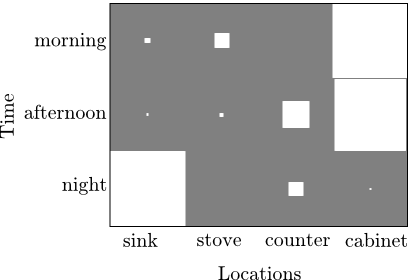
\includegraphics[width=0.6\textwidth]{images/absent_groundtruth.png}
\caption[Simulated object location ground truth distribution]{Simulated object location ground truth distribution.
The x-axis represents the locations the y axis represents the timezones. The size of the white box indicates the probability of the object presence.}
\label{absent-gt}
\end{figure}

From the ground truth we can observe that there is higher probability to find the object in the sink during night time and in the cabinet during the other time periods. We need to develop models which can learn these temporal patterns from the observations

\section{Evaluation}

\todo[inline]{TODO}

We compare the Dirichlet-Categorical-Bernoulli model with the Hierarchical-Dirichlet-Categorical model explained in \ref{sec: HDCM}. We compare the ground truth dirichlet probabilities, used to generate the simulated dataset and the learned probabilities and evaluate the performance of the learning. 
We use the adopted  Bhattacharyya distance \cite{rauber2008bhattacharyya} to quantify the similarity between the simulated and the learned Dirichlet distribution.
\begin{figure}
    \centering
    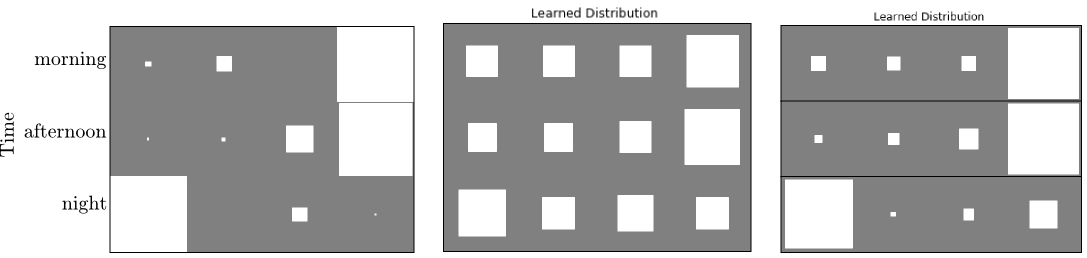
\includegraphics[width=\textwidth]{images/absent_learned.png}
       
    \begin{minipage}[t]{.35\textwidth}
    %\centering
    \subcaption{Ground Truth}\label{fig:absent-gt}
    \end{minipage}%
    \begin{minipage}[t]{.3\textwidth}
    %\centering
    \subcaption{HDC model}\label{fig:absent-hdcm}
    \end{minipage}
    \begin{minipage}[t]{.25\textwidth}
    %\centering
    \subcaption{HDCB model}\label{fig:absent-hdcmb}
    \end{minipage}

\caption[Model Evaluation of HDC and HDCB ]{Model Evaluation: \ref{fig:absent-gt} is ground truth of the distribution. \ref{fig:absent-hdcm} is the learned distribution using the HDC model. \ref{fig:absent-hdcmb} is the learned distribution using the HDCB  model }
        \label{fig:absent-eval}
    
\end{figure}


\begin{figure}[htp]
\centering
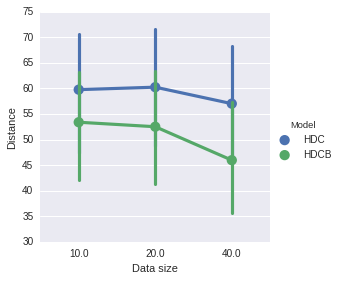
\includegraphics[width=\textwidth]{images/bhatta-distance.png}
\caption[Model evaluation : Bhattacharyya distance]{Bhattacharyya distance between the ground truth and the learned distributions for different size of training data. }
\label{}
\end{figure}



